\chapter{Representaciones del comportamiento}\label{cha:representacion_comportamiento}

\AddToShipoutPictureBG*{\put(0,0){%
        \parbox[b][\paperheight]{\paperwidth}{%
            \vfill
            \centering
            
\includegraphics[width=\paperwidth,height=\paperheight,keepaspectratio]{%
                figuras/caratulas/representacion_del_comportamiento.jpg}\vfill
        }}}

\AddToShipoutPicture*{
    \begin{tikzpicture}[overlay, remember picture]
        \fill[white, opacity=0.75] (20, 24) rectangle (1, 20);
    \end{tikzpicture}}

\clearpage

\section{Niveles de descripción del comportamiento}\label{sec:niveles_descripcion_comportamiento}

Existen diferentes niveles de granularidad para describir el comportamiento animal \cite{datta_computational_neuroethology}.
Esta granularidad depende del nivel de detalle que se utilice en la caracterización anatómica, funcional y temporal del sistema. Por ejemplo, la locomoción de un animal se puede describir desde el nivel celular como contracciones y relajaciones de fibras musculares, o a grandes rasgos simplemente determinando si el animal está quieto o en movimiento.

En este sentido, nosotros utilizamos métricas que describen el comportamiento de manera global, en la escala temporal de la duración de la tarea motora (\autoref{fig:capitulo3_representacion_comportamiento}). Estas métricas son un resumen general del rendimiento y de la ejecución de una prueba, sin entrar en demasiados detalles sobre lo que sucedió a pequeña escala. Las métricas también se conocen como puntajes o \textit{scores}, pues son la principal manera de evaluar el rendimiento de una tarea realizada. A su vez, describir el comportamiento animal usando métricas, que resumen lo ocurrido en una tarea entera, permite analizar patrones de variación del comportamiento a escalas temporales más largas (por ejemplo, permite estudiar variaciones a lo largo de varias pruebas sucesivas y a lo largo de días de entrenamiento, revelando fenómenos de fatiga, aprendizaje, deterioro neurológico, entre otros).

\begin{figure}[htbp]
    \centering
    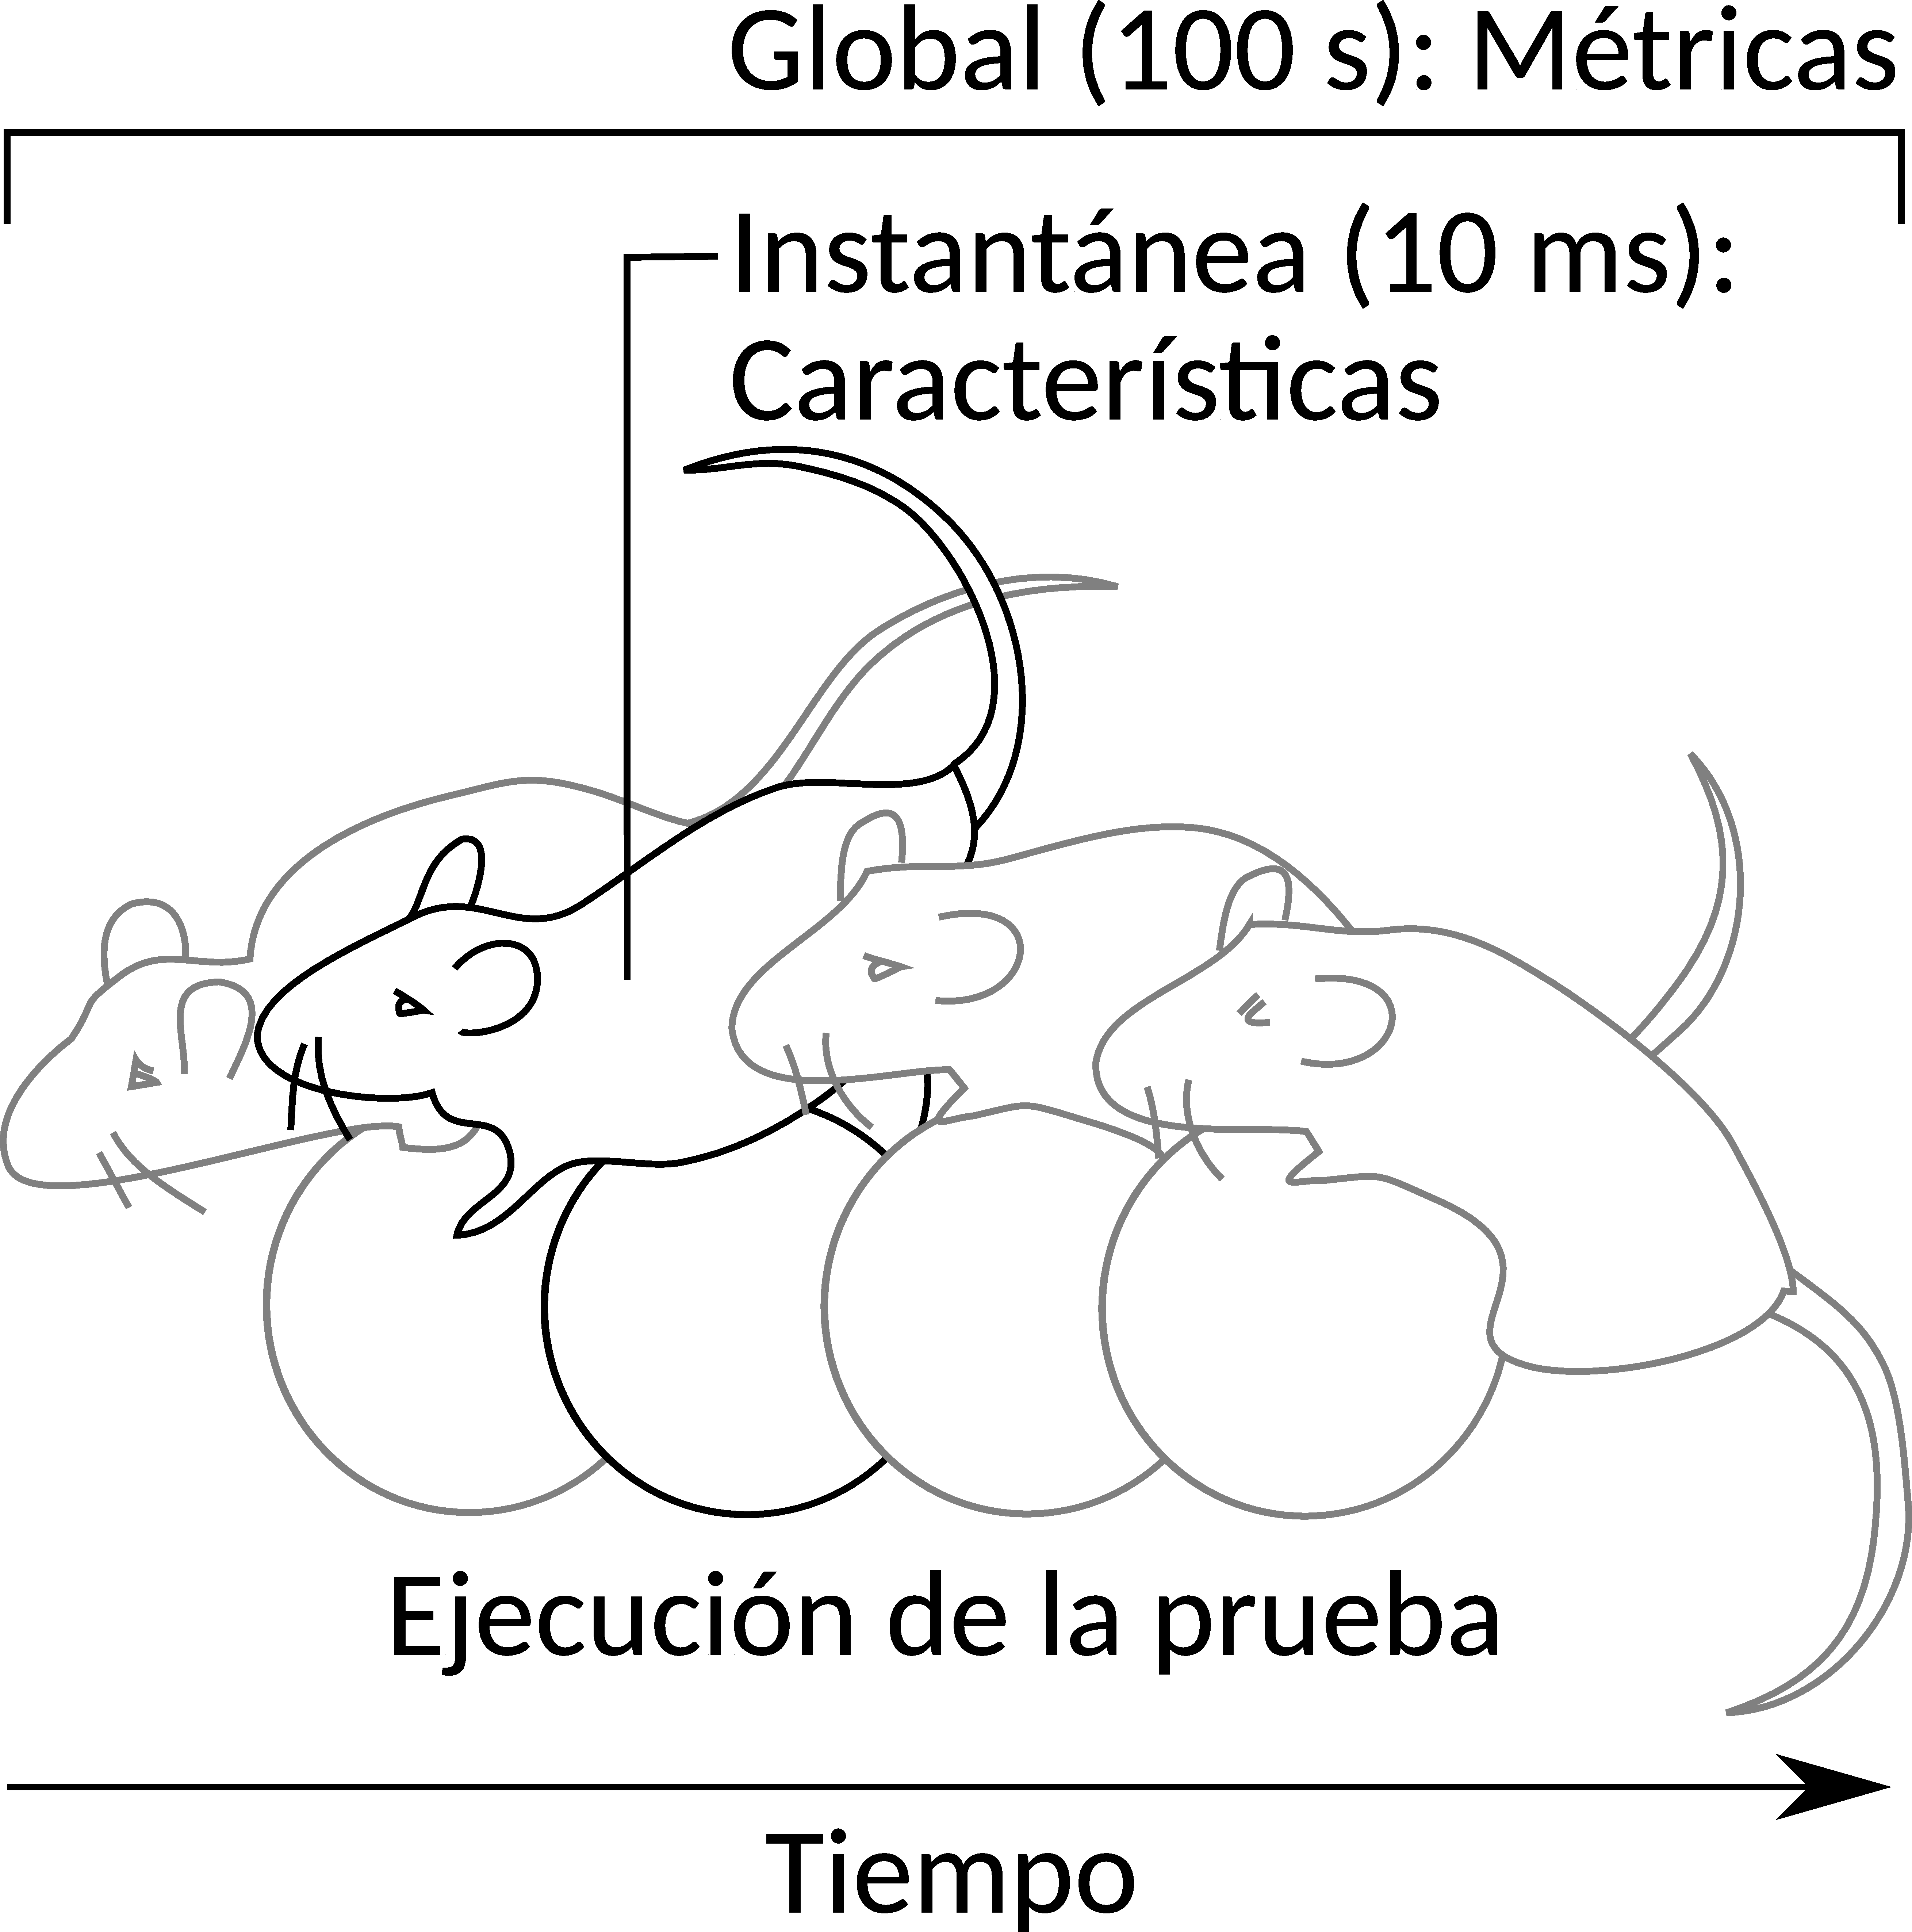
\includegraphics[width=0.45\linewidth]{figuras/capitulo3/representacion_comportamiento.pdf}
    \caption{\textbf{Escalas temporales en la descripción del comportamiento.} Ilustración de diferentes niveles de descripción del comportamiento animal, según la escala temporal de observación.}
    \label{fig:capitulo3_representacion_comportamiento}
\end{figure}

Formalmente, una métrica es una función que toma una realización de una prueba y devuelve un valor numérico
\begin{equation*}
    \text{Métrica comportamental}: \text{Prueba realizada} \mapsto \text{Valor} \in \mathbb{R}.
\end{equation*}

Por ejemplo, la latencia a caer es una de las métricas clásicas utilizadas para cuantificar el rendimiento en la tarea rotarod con aceleración. Para calcularla simplemente se determina el tiempo en que tarda un ratón en caerse del cilindro rotarod en una prueba. En la práctica, restringimos además la duración de cada prueba a un máximo de $300$ s, por lo que la latencia a caer es menor o igual a ese valor.

\clearpage

De acuerdo a los valores observados de latencia a caer, separamos a los individuos en dos grupos de rendimiento: 7 ratones de rendimiento bajo y 3 ratones de rendimiento alto (\autoref{fig:capitulo3_probabilidad_caer_por_rendimiento}). Los promedios de la latencia a caer de cada grupo se mantuvieron separados por una brecha de alrededor de 100 s (equivalente a entre 2 y 3 desviaciones estándar) durante todo el entrenamiento. Esta separación en grupos de rendimiento según la latencia a caer no se explica por el peso, sexo ni edad de los ratones, ya que estas condiciones eran homogéneas entre individuos. Sin embargo, podría depender del ritmo circadiano de los individuos, entre otros factores, si es que son más activos en diferentes momentos del día, ya que las pruebas rotarod se realizaron por la mañana de forma regular.

\begin{figure}[htbp]
    \centering
    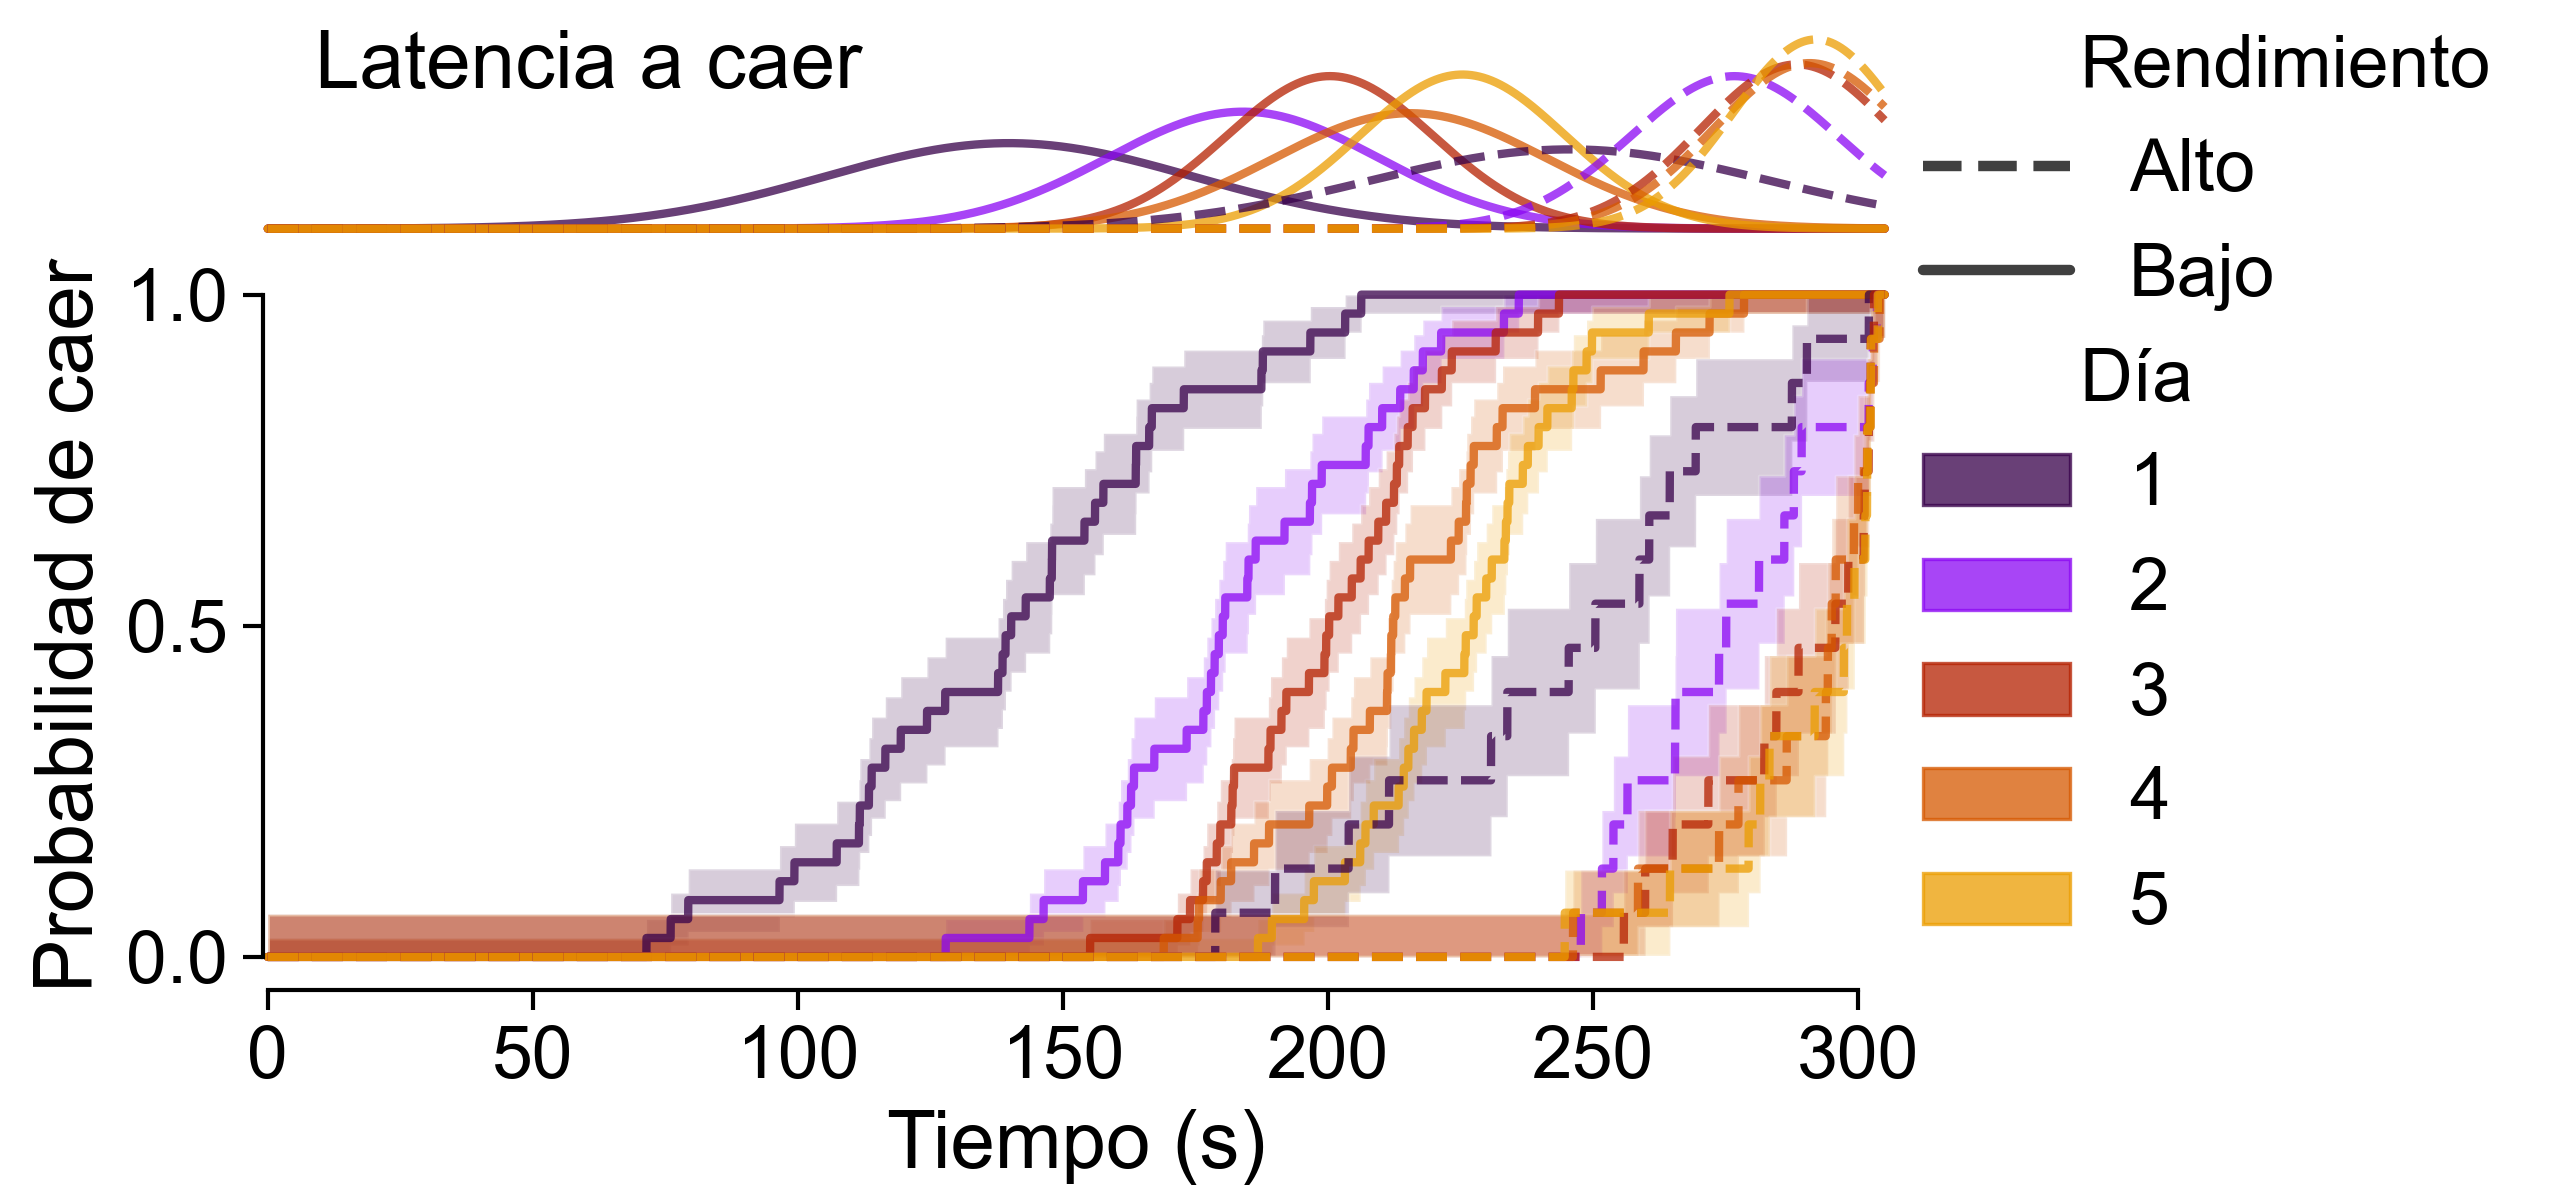
\includegraphics[width=0.8\linewidth]{figuras/capitulo3/probabilidad_caer_por_rendimiento.png}
    \caption{\textbf{Distribución de la latencia a caer.} (Abajo) Probabilidad de caer en un determinado tiempo de una prueba. (Arriba) Distribuciones de la latencia a caer.
        La latencia a caer aumenta con el día de entrenamiento y se observan dos grupos de ratones de diferente rendimiento.}
    \label{fig:capitulo3_probabilidad_caer_por_rendimiento}
\end{figure}

Otra métrica que se puede calcular es el valor promedio que adopta una característica comportamental durante una prueba. Sin embargo, la latencia a caer varía mucho (diferencias de 100 s) entre individuos, ya sea por su nivel de rendimiento o por su estadío de entrenamiento, por lo que tenemos registros bajo diferentes condiciones experimentales (la velocidad del cilindro rotarod aumenta con el tiempo). Por lo tanto, el promedio de la característica comportamental debe calcularse sobre tiempos donde se tengan registros de los individuos, bajo condiciones experimentales similares. Solamente 3 de las 250 pruebas realizadas tienen latencias a caer menores a 100 s, con una latencia a caer mínima observada de 70 s. Por estos motivos, calculamos los promedios dentro de los primeros 100 s de la tarea. También calculamos la pendiente con la que cambian las características de los pasos en estos primeros 100 s y el error en su ejecución.

Las características (conocidas también como \textit{features}) describen el comportamiento de manera más detallada. Las características comportamentales proporcionan información a escalas de tiempo sub-segundo, dependiendo de la resolución temporal experimental. Estas brindan una explicación detallada de la ejecución de una prueba, instante a instante, de manera aproximadamente continua. A su vez, estas descripciones a escalas de tiempo cortas pueden integrarse de diferentes maneras para dar origen a múlitples métricas comportamentales, que describen el comportamiento de manera global.

Un ejemplo de características comportamentales son las posiciones de las partes del cuerpo de los ratones, en nuestro caso medidas con una resolución temporal de $10$ ms. Otras características pueden ser los espectros de frecuencia \textit{wavelet} obtenidos de las partes del cuerpo de los ratones, u otras señales biofísicas. En particular, nosotros utilizaremos además de las posiciones de los marcadores, características que describen los pasos realizados por los ratones sobre el cilindro rotarod. Específicamente, las alturas mínima y máxima comprendidas en los pasos, su amplitud, velocidad instantánea, desfasaje entre las patas traseras y frecuencia entre pasos consecutivos de una misma pata.

Formalmente, una característica es una función que toma un tiempo determinado en una prueba y devuelve un valor numérico
\begin{equation*}
    \text{Característica comportamental}: \text{Tiempo} \mapsto \text{Valor} \in \mathbb{R}.
\end{equation*}

Por último, un conjunto de características comportamentales constituye una representación comportamental. El proceso de selección de características para representar el comportamiento depende de restricciones físicas, computacionales, experimentales o presupuestarias de cada laboratorio. En general, es conveniente utilizar una representación que sea sencilla y fácil de interpretar. Y que además incluya una cantidad características lo suficientemente grande para explicar detalladamente el comportamiento animal, pero lo suficientemente pequeña como para que el análisis sea computacionalmente eficiente
\begin{equation*}
    \text{Representación comportamental} = \{\text{Características comportamentales}\}.
\end{equation*}

A su vez, la representación comportamental elegida condiciona el tipo de información que se puede extraer en el análisis de la tarea. También podríamos representar el comportamiento usando un conjunto de métricas, como la latencia a caer, para describir el comportamiento en la escala temporal de la duración de las pruebas rotarod. Sin embargo, en este trabajo estudiaremos más adelante representaciones del comportamiento a escala temporal sub-segundo, para describir el comportamiento de los ratones durante cada instante de la tarea rotarod y construir mapas de comportamiento de dimensión reducida.

Finalmente, la ejecución de una prueba rotarod, vista a través de una característica en particular, son los valores de esa característica observados experimentalmente durante la tarea
\begin{align*}
    \text{Ejecución de una Prueba según una Característica} = & \ \{ \text{Característica(Tiempo)}         \\
                                                              & \ \text{para cada Tiempo de la Prueba} \}.
\end{align*}

A su vez, podemos juntar todas las características observadas durante una prueba, dentro de una representación comportamental dada, y llamar ejecución a este conjunto de observaciones
\begin{align*}
    \text{Ejecución de una Prueba} = & \ \{ \text{Característica(Tiempo)}               \\
                                     & \ \text{para cada Tiempo de la Prueba}           \\
                                     & \ \text{y para cada Característica}              \\
                                     & \ \text{de la Representacióń comportamental} \}.
\end{align*}

\clearpage

\section{Variación en las métricas por rendimiento y entrenamiento}\label{sec:variacion_metricas_grupo_rendimiento_dia_entrenamiento}

\begin{figure}[htbp]
    \centering
    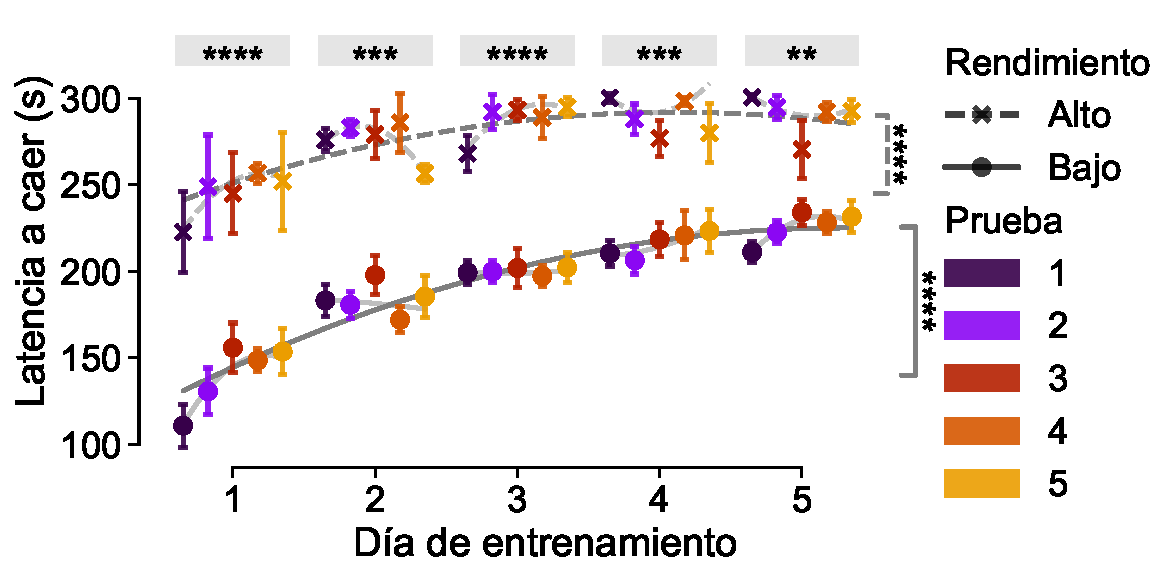
\includegraphics[width=0.8\linewidth]{figuras/capitulo3/latencia_por_prueba_por_rendimiento.pdf}
    \caption{\textbf{Latencia a caer por día y grupo de rendimiento.} La latencia a caer aumenta con el día de entrenamiento y se conserva una brecha entre los grupos de rendimiento.
        Los puntos muestran el promedio por grupo de rendimiento y las barras son el error estándar del promedio.
        Los rectángulos grises superiores indican los p-valores T-test entre grupos de rendimiento para cada día.
        Los corchetes en el margen derecho indican, para cada grupo de rendimiento, los p-valores \textit{one-way} ANOVA agrupando por día de entrenamiento.}
    \label{fig:capitulo3_latencia_por_prueba_por_rendimiento}
\end{figure}

Clásicamente, la latencia a caer es la métrica utilizada para evaluar el rendimiento y el aprendizaje motor en la tarea rotarod (\autoref{fig:capitulo3_latencia_por_prueba_por_rendimiento}). Nos interesa estudiar también cómo evolucionan otras métricas en función del día de entrenamiento y el grupo de rendimiento. Para ello, utilizaremos el Promedio$\{\xi\}$ (\autoref{fig:capitulo3_metricas_promedio}) y la Pendiente$\{\xi\}$ (\autoref{fig:capitulo3_metricas_pendiente}) de diferentes características de pasos $\xi$ durante los primeros 100 s de la tarea. Además, utilizaremos la raíz del error cuadrático medio RMSE$\{\xi\}$ (\autoref{fig:capitulo3_metricas_rmse}), para evaluar efectos del aprendizaje en la ejecución de la tarea. Calculamos este error como
\begin{equation*}
    \mathrm{RMSE}\{\xi\} = \sqrtexplained{%
    \langle \ \ \; \underbrace{[\hat{\mu}_{\xi}(t) - \mu^{\mathrm{fit}}_{\xi}(t)]^2}
    _{\substack{
            \text{Desviaciones}\\
            \text{respecto de una}\\
            \text{ejecución suave}
        }} + \underbrace{\hat{\sigma}_{\xi}^2(t)}
    _{\substack{
        \text{Varianza de}\\
        \text{la ejecución}\\
        \text{observada}
    }} \rangle
    } \, .
\end{equation*}

Identificamos dos términos que contribuyen al error de ejecución RMSE. Por un lado, un término de desviaciones respecto de la tendencia ajustada ($[\hat{\mu}_{\xi}(t) - \mu^{\mathrm{fit}}_{\xi}(t)]^2$), que representa la ``exactitud'' de la estrategia de locomoción. Y, por otro lado, un término de varianza ($\hat{\sigma}_{\xi}^2(t)$), que se interpreta como la ``precisión'' de la estrategia motora.

De esta manera, el error RMSE captura eventos en los que el ratón cambia súbitamente de estrategia de locomoción (por ejemplo, si tropieza o resbala), pues estos eventos producen desvíos grandes en $\hat{\mu}_x$ respecto de la tendencia ajustada $\mu^{\mathrm{fit}}_x$. Esto se debe a que la tendencia ajustada $\mu^{\mathrm{fit}}_{\xi}$ (polinomio de grado 3) es mucho más suave que $\hat{\mu}_{\xi}$, como función del tiempo $t$, por lo que no varía bruscamente frente a estos eventos de cambio de estrategia. Además, el error RMSE toma en cuenta la variablidad intrínseca de la característica $\xi$, a través de su varianza $\hat{\sigma}_{\xi}^2(t)$. Intuitivamente, el error RMSE cuantifica qué tanto se desvía la estrategia de locomoción del ratón, respecto de una estrategia que varía de manera suave y que se ejecuta de manera precisa.

Para el cálculo de las métricas Promedio, Pendiente y RMSE, promediamos las características $\xi$ las patas izquierda y derecha. De esta manera eliminamos las variaciones por lateralidad que puedan tener los ratones, por ejemplo por tener una pata dominante. Al promediar las características entre las patas ignoramos también estrategias de comportamiento asimétricas, por ejemplo si el ratón se mueve inclinado respecto de la horizontal del cilindro. Esto lo hacemos para simplificar esta parte del análisis, a pesar de la pérdida de información detallada de la estrategia de locomoción.

Respecto a los resultados obtenidos (Figuras \ref{fig:capitulo3_metricas_promedio}, \ref{fig:capitulo3_metricas_pendiente} y \ref{fig:capitulo3_metricas_rmse} suplementarias), en general el grupo de 7 ratones de bajo rendimiento muestra cambios estadísticamente más significativos durante el entrenamiento, comparado con el grupo de 3 ratones de alto rendimiento (\autoref{tab:pvalores-anova}). Esta mayor significancia estadística se explica tanto por el mayor número de ratones en el grupo de bajo rendimiento, como también por la mayor magnitud de los cambios en los valores de las métricas a lo largo de los días de entrenamiento, frente a las fluctuaciones intra-día. En particular, en las métricas Promedio, Pendiente y RMSE calculadas a partir de la Altura mínima, Altura máxima y Frecuencia muestran los cambios más significativos con el aprendizaje, para el grupo de bajo rendimiento. Mientras que para el grupo de alto rendimiento, las métricas Promedio y RMSE (no así la Pendiente) presentan los cambios más significativos cuando son calculadas a partir de la Altura máxima y la Frecuencia de los pasos.

En general, las mayores variaciones interprueba en las métricas ocurren más frecuentemente en la prueba D1T2, respecto de la prueba inmediatamente anterior D1T1 (\autoref{tab:variacion-interpureba}). Más detalladamente, en la prueba D1T2 se observaron las mayores variaciones en 5 de las 6 métricas RMSE, en 2 de las 6 métricas Promedio y en ninguna de las métricas Pendiente. Finalmente, las métricas Latencia a caer y Promedio\{Amplitud\} sufren su mayor cambio en la prueba D2T1, respecto de la prueba inmediatamente anterior D1T5 (\autoref{tab:variacion-interpureba}).

De esta manera, la mayoría de las métricas RMSE, la mitad de las Promedio y la Latencia a caer sufren cambios significativos de manera relativamente temprana, durante el comienzo del primer y segundo día del proceso de entrenamiento. Por su parte, la mayoría de las métricas Pendiente sufren cambios significativos más tardíos, ocurriendo las mayores variaciones en la prueba D3T1 (3 de las 6 métricas) y en la prueba D5T1 (2 de las 6 métricas). Además, la otra mitad de las métricas Promedio y una de las RMSE sufren cambios tardíos.

En cuanto a las diferencias entre los grupos de rendimiento, estas son más significativas al comienzo (D1 y D2) y al final (D5) del entrenamiento, según la mayoría de las métricas (\autoref{tab:pvalores-t-test}). Todas las métricas Promedio y 4 de las 6 métricas RMSE muestran diferencias significativas entre los grupos de rendimiento en todos los días. En cuanto a las métricas Pendiente, se observan diferencias significativas entre los grupos de rendimiento en 5 de estas 6 métricas en el día D1, en 3 de 6 en el día D2 y en 4 de 6 en el día D5. En particular, las métricas Pendiente\{Altura máxima\} y Pendiente\{Desfasaje\} comienzan con diferencias significativas entre los grupos de rendimiento en el día D1, y estas diferencias se hacen menos significativas con el entrenamiento. En general, la característica Frecuencia muestra diferencias menos significativas que el resto de las características, para todas las métricas.

En resumen, el método más tradicional de representación del comportamiento, la métrica de latencia a caer, captura el progreso de los animales durante el entrenamiento y también las diferencias entre animales según su aptitud física previa. Adicionalmente, conseguimos definir otras métricas que describir de manera global cómo se desempeñan los ratones en la tarea. De esta manera aportamos más información sobre el comportamiento de los ratones. Vimos que no solo aumenta la latencia a caer con el entrenamiento, sino que también aumentan la altura a la que los ratones dan pasos sobre el cilindro rotarod, mientras que la amplitud y la velocidad de los pasos se reduce (\autoref{fig:capitulo3_metricas_promedio}). Además, los ratones de bajo rendimiento aprenden a mantenerse más arriba del cilindro, reduciendo la tendencia a que la rotación del cilindro los arrastre hacia abajo (\autoref{fig:capitulo3_metricas_pendiente} Pendiente de la Altura mínima y de la Altura máxima). Registramos que los errores en las ejecuciones comportamentales de los ratones se reduce con el entrenamiento (\autoref{fig:capitulo3_metricas_rmse}). Observamos que la mayoría de los cambios más significativos en estas métricas se dan en la segunda prueba del primer día de entrenamiento, mostrando la rapidez con la que los ratones se adaptan a nuevos entornos. El desfasaje entre los pasos de las patas traseras no cambia significativamente durante el entrenamiento.

A su vez, la mayoría de las métricas alternativas estudiadas separan a los ratones en 2 grupos de rendimiento: 7 ratones de bajo rendimiento y 3 ratones de alto rendimiento. Estos grupos de rendimiento se definieron con base a la latencia a caer exhibida por los ratones, habiendo una maracada brecha desde el primer día de entrenamiento que se mantuvo hasta el día cinco, el último día de entrenamiento registrado.

Las variaciones de las métricas alternativas a la latencia a caer son más visibles en el grupo de ratones de bajo rendimiento. Sin embargo, debido a la alta variabilidad intra-día de las métricas, al realizar un ANOVA de las métricas a lo largo del entrenamiento, solamente la Altura mínima, la Altura máxima y la Frecuencia de los pasos cambia de manera estadísticamente significativa, de manera más consistente al calcular su Promedio, Pendiente y error de ejecución RMSE durante los primeros 100 s de las pruebas rotarod. Esto no quita que la existencia de cambios, aunque sea sutiles, en el resto de las métricas, aunque quedan enmascarados por la alta variabilidad entre pruebas en un mismo día (Figuras \ref{fig:capitulo3_metricas_promedio}, \ref{fig:capitulo3_metricas_pendiente} y \ref{fig:capitulo3_metricas_rmse} suplementarias). Respecto a la variabilidad intra-día, esta podría deberse a un proceso de fatiga o a un aprendizaje a corta escala temporal, pero para determinar su origen hacen falta más estudios teniendo en cuenta esos factores.

En el capítulo siguiente introducimos mapas de comportamiento usando el algoritmo UMAP de reducción de la dimensión. Esta es una manera de visualizar, de manera resumida, la información de un conjunto de múltiples características comportamentales. Decimos que los conjuntos de características de los que partimos son de dimensión alta (en nuestro caso, entre 30 y 50 dimensiones), en contraste con el mapa UMAP obtenido, que es una representación resumida del sistema, en una proyección de 2 dimensiones.

\begin{table}[htbp]
    \centering
    \begin{tabular}{clcc}
                                                                      &                   & \multicolumn{2}{c}{\textbf{Rendimiento}}                               \\ \cline{3-4}
                                                                      & \textbf{Métricas} & \textbf{Bajo}                            & \textbf{Alto}               \\ \cline{2-4}
                                                                      & Latencia a caer   & $\mathbf{1\times 10^{-30}}$              & $\mathbf{1\times 10^{-6}}$  \\ \cline{2-4}
        \multirow{6}{*}{\rotatebox[origin=c]{90}{\textbf{Promedio}}}  & Altura mínima     & $\mathbf{5\times 10^{-3}}$               & 0.12                        \\
                                                                      & Altura máxima     & $\mathbf{1\times 10^{-7}}$               & $\mathbf{9\times 10^{-3}}$  \\
                                                                      & Amplitud          & 0.34                                     & 0.42                        \\
                                                                      & Velocidad         & 0.49                                     & 0.49                        \\
                                                                      & Desfasaje         & 0.25                                     & \textbf{0.034}              \\
                                                                      & Frecuencia        & $\mathbf{6\times 10^{-4}}$               & $\mathbf{10\times 10^{-4}}$ \\ \cline{2-4}
        \multirow{6}{*}{\rotatebox[origin=c]{90}{\textbf{Pendiente}}} & Altura mínima     & $\mathbf{2\times 10^{-5}}$               & 0.44                        \\
                                                                      & Altura máxima     & $\mathbf{4\times 10^{-11}}$              & 0.53                        \\
                                                                      & Amplitud          & \textbf{0.035}                           & 0.51                        \\
                                                                      & Velocidad         & 0.068                                    & 0.69                        \\
                                                                      & Desfasaje         & 0.61                                     & \textbf{0.011}              \\
                                                                      & Frecuencia        & \textbf{0.011}                           & 0.99                        \\ \cline{2-4}
        \multirow{6}{*}{\rotatebox[origin=c]{90}{\textbf{RMSE}}}      & Altura mínima     & 0.072                                    & 0.065                       \\
                                                                      & Altura máxima     & $\mathbf{5\times 10^{-6}}$               & $\mathbf{5\times 10^{-4}}$  \\
                                                                      & Amplitud          & 0.072                                    & 0.081                       \\
                                                                      & Velocidad         & 0.46                                     & 0.19                        \\
                                                                      & Desfasaje         & 0.055                                    & 0.21                        \\
                                                                      & Frecuencia        & $\mathbf{4\times 10^{-4}}$               & \textbf{0.032}
    \end{tabular}
    \caption{\textbf{Cambios más significativos en el grupo de bajo rendimiento.} p-valores \textit{one-way} ANOVA para medir cambios a lo largo de los días de entrenamiento, para cada grupo de rendimiento. Los p-valores estadísticamente significativos se indican en negrita.}
    \label{tab:pvalores-anova}
\end{table}

\begin{table}[htbp]
    \centering
    \begin{tabular}{clcccc}
                                                                      &                                   & \multicolumn{4}{c}{\textbf{Mayor variación interprueba}}                                                                  \\ \cline{3-6}
                                                                      & \textbf{Métricas}                 & \textbf{Pruebas}                                         & \textbf{Nominal} & \textbf{Porcentual (\%)} & \textbf{Z-score} \\ \cline{2-6}
                                                                      & Latencia a caer (s)               & \bf D2T1                                                 & 30(16)           & 24(13)                   & 1.8              \\ \cline{2-6}
        \multirow{6}{*}{\rotatebox[origin=c]{90}{\textbf{Promedio}}}  & Altura mínima (mm)                & \bf D1T2                                                 & 3.2(2.3)         & 47(33)                   & 1.4              \\
                                                                      & Altura máxima (mm)                & \bf D1T2                                                 & 2.6(0.9)         & 60(20)                   & 3.0              \\
                                                                      & Amplitud (mm)                     & D2T1                                                     & -2.0(2.2)        & -60(67)                  & 0.9              \\
                                                                      & Velocidad (mm s$^{-1}$)           & D4T1                                                     & -28(28)          & -66(66)                  & 1.0              \\
                                                                      & Desfasaje (vueltas)               & D3T5                                                     & 0.012(0.015)     & 29(36)                   & 0.8              \\
                                                                      & Frecuencia (Hz)                   & \bf D4T5                                                 & -0.14(0.06)      & -30(13)                  & 2.3              \\ \cline{2-6}
        \multirow{6}{*}{\rotatebox[origin=c]{90}{\textbf{Pendiente}}} & Altura mínima (mm hs$^{-1}$)      & \bf D3T1                                                 & 5.1(2.1)         & 58(24)                   & 2.4              \\
                                                                      & Altura máxima (mm hs$^{-1}$)      & \bf D2T4                                                 & 1.2(0.6)         & 34(16)                   & 2.1              \\
                                                                      & Amplitud (mm hs$^{-1}$)           & \bf D3T1                                                 & -4.8(1.7)        & -77(27)                  & 2.9              \\
                                                                      & Velocidad (mm s$^{-1}$ hs$^{-1}$) & \bf D3T1                                                 & -81(25)          & -93(29)                  & 3.2              \\
                                                                      & Desfasaje (vueltas hs$^{-1}$)     & \bf D5T1                                                 & -0.085(0.051)    & -73(43)                  & 1.7              \\
                                                                      & Frecuencia (Hz hs$^{-1}$)         & \bf D5T1                                                 & -0.29(0.08)      & -80(22)                  & 3.6              \\ \cline{2-6}
        \multirow{6}{*}{\rotatebox[origin=c]{90}{\textbf{RMSE}}}      & Altura mínima (mm)                & \bf D1T2                                                 & -1.4(0.3)        & -75(17)                  & 4.3              \\
                                                                      & Altura máxima (mm)                & \bf D1T2                                                 & -1.1(0.5)        & -47(22)                  & 2.1              \\
                                                                      & Amplitud (mm)                     & \bf D1T2                                                 & -1.0(0.4)        & -60(22)                  & 2.7              \\
                                                                      & Velocidad (mm s$^{-1}$)           & \bf D1T2                                                 & -12(5)           & -68(29)                  & 2.3              \\
                                                                      & Desfasaje (vueltas)               & \bf D3T4                                                 & -0.010(0.005)    & -44(21)                  & 2.0              \\
                                                                      & Frecuencia (Hz)                   & \bf D1T2                                                 & -0.20(0.07)      & -58(20)                  & 2.9
    \end{tabular}
    \caption{\textbf{Mayoría de cambios ocurren en la prueba D1T2.} Pruebas en las que se observó la mayor variación en el Z-score de las métricas, respecto de la prueba inmediatamente anterior. Se muestran los resultados del grupo de ratones de bajo rendimiento. Las pruebas con Z-scores mayores a 1 se indican en negrita. El símbolo D$i$T$j$ denota la prueba $j$ del día $i$.}
    \label{tab:variacion-interpureba}
\end{table}

\begin{table}[htbp]
    \centering
    \begin{tabular}{clccccc}
                                                                      &                   & \multicolumn{5}{c}{\textbf{Día de entrenamiento}}                                                                                                                     \\ \cline{3-7}
                                                                      & \textbf{Métricas} & \textbf{D1}                                       & \textbf{D2}                & \textbf{D3}                & \textbf{D4}                & \textbf{D5}                \\ \cline{2-7}
                                                                      & Latencia a caer   & $\mathbf{3\times 10^{-5}}$                        & $\mathbf{3\times 10^{-4}}$ & $\mathbf{5\times 10^{-5}}$ & $\mathbf{4\times 10^{-4}}$ & $\mathbf{2\times 10^{-3}}$ \\ \cline{2-7}
        \multirow{6}{*}{\rotatebox[origin=c]{90}{\textbf{Promedio}}}  & Altura mínima     & $\mathbf{5\times 10^{-5}}$                        & $\mathbf{2\times 10^{-6}}$ & $\mathbf{9\times 10^{-6}}$ & $\mathbf{2\times 10^{-4}}$ & $\mathbf{1\times 10^{-4}}$ \\
                                                                      & Altura máxima     & $\mathbf{3\times 10^{-3}}$                        & $\mathbf{2\times 10^{-6}}$ & $\mathbf{2\times 10^{-4}}$ & $\mathbf{3\times 10^{-5}}$ & $\mathbf{1\times 10^{-5}}$ \\
                                                                      & Amplitud          & $\mathbf{2\times 10^{-3}}$                        & $\mathbf{1\times 10^{-5}}$ & $\mathbf{3\times 10^{-6}}$ & $\mathbf{4\times 10^{-4}}$ & $\mathbf{2\times 10^{-4}}$ \\
                                                                      & Velocidad         & $\mathbf{2\times 10^{-3}}$                        & $\mathbf{5\times 10^{-5}}$ & $\mathbf{2\times 10^{-5}}$ & $\mathbf{5\times 10^{-4}}$ & $\mathbf{2\times 10^{-4}}$ \\
                                                                      & Desfasaje         & $\mathbf{9\times 10^{-3}}$                        & $\mathbf{2\times 10^{-3}}$ & $\mathbf{2\times 10^{-3}}$ & $\mathbf{2\times 10^{-3}}$ & $\mathbf{2\times 10^{-4}}$ \\
                                                                      & Frecuencia        & \textbf{0.012}                                    & \textbf{0.022}             & \textbf{0.010}             & \textbf{0.012}             & \textbf{0.022}             \\ \cline{2-7}
        \multirow{6}{*}{\rotatebox[origin=c]{90}{\textbf{Pendiente}}} & Altura mínima     & $\mathbf{8\times 10^{-3}}$                        & \textbf{0.032}             & 0.65                       & 0.17                       & \textbf{0.017}             \\
                                                                      & Altura máxima     & \textbf{0.016}                                    & 0.25                       & 0.15                       & 0.37                       & 0.084                      \\
                                                                      & Amplitud          & $\mathbf{4\times 10^{-3}}$                        & \textbf{0.021}             & 0.31                       & 0.073                      & $\mathbf{3\times 10^{-3}}$ \\
                                                                      & Velocidad         & $\mathbf{3\times 10^{-3}}$                        & \textbf{0.015}             & 0.22                       & 0.052                      & $\mathbf{3\times 10^{-3}}$ \\
                                                                      & Desfasaje         & \textbf{0.028}                                    & 0.11                       & 0.39                       & 0.48                       & 0.49                       \\
                                                                      & Frecuencia        & 0.59                                              & 0.64                       & 0.65                       & 0.57                       & \textbf{0.021}             \\ \cline{2-7}
        \multirow{6}{*}{\rotatebox[origin=c]{90}{\textbf{RMSE}}}      & Altura mínima     & $\mathbf{2\times 10^{-3}}$                        & $\mathbf{1\times 10^{-5}}$ & $\mathbf{1\times 10^{-3}}$ & $\mathbf{6\times 10^{-4}}$ & $\mathbf{4\times 10^{-3}}$ \\
                                                                      & Altura máxima     & \textbf{0.013}                                    & $\mathbf{3\times 10^{-5}}$ & $\mathbf{5\times 10^{-3}}$ & $\mathbf{3\times 10^{-4}}$ & $\mathbf{2\times 10^{-3}}$ \\
                                                                      & Amplitud          & $\mathbf{2\times 10^{-3}}$                        & $\mathbf{3\times 10^{-5}}$ & $\mathbf{4\times 10^{-4}}$ & $\mathbf{1\times 10^{-3}}$ & $\mathbf{2\times 10^{-3}}$ \\
                                                                      & Velocidad         & $\mathbf{5\times 10^{-4}}$                        & $\mathbf{3\times 10^{-4}}$ & $\mathbf{2\times 10^{-4}}$ & $\mathbf{5\times 10^{-4}}$ & $\mathbf{2\times 10^{-3}}$ \\
                                                                      & Desfasaje         & 0.58                                              & 0.49                       & 0.67                       & 0.95                       & 0.70                       \\
                                                                      & Frecuencia        & 0.49                                              & 0.61                       & 0.26                       & 0.61                       & 0.90
    \end{tabular}
    \caption{\textbf{Mayoría de métricas separan los grupos de rendimiento.} p-valores T-test entre grupos de rendimiento. Los p-valores estadísticamente significativos se indican en negrita. El símbolo D$i$ denota el día $i$.}
    \label{tab:pvalores-t-test}
\end{table}